\begin{frame}{从反问题到能观测不等式}
  反问题是指根据事物表现出来的\textcolor{magenta}{局部信息},来推断事物\textcolor{magenta}{整体信息}.
  \begin{figure}
    \begin{tikzpicture}[scale=0.7]
      \fill[blue!90!black] plot[smooth cycle] coordinates{(0,0) (4,0) (2.5,2.5) (-1,2.5)};
      \fill[magenta] (0.5,0.5) ellipse (0.5 and 0.375);
      \fill[magenta] (0.9,2.1) ellipse (0.5 and 0.375);
      \fill[magenta] (2.5,0.8) ellipse (0.5 and 0.375);
      \draw (2,-0.3) node[below]{$\Omega$};
      \draw[->] (4-0.15,2) to[out=180,in=40]  (0.5,0.5);
      \draw[->] (4-0.1,2+0.1) to[out=150, in=30] (0.9,2.1);
      \draw[->] (4-0.15,2-0.1) to[out=-120, in=10] (2.5,0.8);
      \draw (4.1,2) node{$\color{magenta}{\omega}$};
      \fill[blue!90!black] (-0.8,-1.5)--(-0.3,-1.5)--(-0.3,-1)--(-0.8,-1)--cycle;
      \draw (-0.3,-1.25) node[right]{\small 非观测区域};
      \fill[magenta] (-0.8+3.5,-1.5)--(-0.3+3.5,-1.5)--(-0.3+3.5,-1)--(-0.8+3.5,-1)--cycle;
      \draw (-0.3+3.5,-1.25) node[right]{\small 观测区域$\color{magenta}\omega$};
    \end{tikzpicture}
  \end{figure}
  设全部区域为${\Omega}$,观测区域为$\color{magenta}{\omega}$,每个时刻和每个位置所提供的信息为$u(t,x)$.那么许多反问题可以归结为下述的\color{red}{能观测不等式}:
  \begin{block}{}
     \[
       \int_{\color{orange}{\Omega}}|u(t,x)|^2\, \mathrm{d}x\le C \int_{0}^{T}\int_{\color{magenta}{\omega}}|u(t,x)|^2\,\mathrm{d}x\mathrm{d}t
     \] 
   \end{block} 
\end{frame}
\begin{frame}{研究对象和内容}
  我们所研究的对象是Korteweg-de Vries (KdV) 方程
  \[
    \partial_t u+\partial_{x}^{3}u=0,\quad u(0,x)=u_0(x) \in L^2(\R)
  \] 
  的解$u(t,x)$并对它建立能观测不等式. 
  
  这里全空间$\Omega=\R$,我们的目标是使得该不等式的
  \begin{itemize}
    \item[(1)] 观测时间$[0,T]$和
    \item[(2)] 观测区域 $\omega$
  \end{itemize}
  越小越好.
\end{frame}
\begin{frame}{研究现状}
  我们用$B_r=\left\{x:|x|\le r\right\} $ 表示半径为$r$的球,  $\R\backslash B_r=\left\{x:|x|>r\right\} $ 表示半径为$r$ 的球外.
  \begin{enumerate}
    \item B. Y. Zhang [SIMA,1992]和J. Bourgain[IMRN,1997]证明了KdV方程的解在两个不同时刻$\omega=\R \backslash  B_r$区域为零时,解恒为零,即$u(t,x)\equiv 0$. 这是定性结果,没有建立定量的不等式.
    \item L. Roiser - B. Y. Zhang [JDE,2009]证明了$\omega=\R \backslash B_r$ (观测区域为球外)的情形的能观测不等式,观测时间是任意一个$[0,T]$的时间段.
    \item Kenig [JFA,2007]证明了在任意一段时间内,解存在某种指数衰减性时,解恒为零.这依然是定性结果.
  \end{enumerate}
\end{frame}
\begin{frame}{研究现状:两点时刻能观测不等式}
  Ze Li - Ming Wang [SIMA,2021]更进一步,证明了任意两个不同时刻球外的能观测不等式:
  \begin{block}{$E=B_{r_1},F=B_{r_2},r_1,r_2>0$}
    \[
      \int_{\R}|u(t,x)|^2\,\mathrm{d}x\le C \left( \int_{\R\backslash \color{magenta}E}|u(t_1,x)|^2\,\mathrm{d}x+\int_{\R \backslash \color{magenta} F}|u(t_2,x)|^2\,\mathrm{d}x \right). 
    \] 
  \end{block}
  可以看到这一新结果不仅使得观测时间变成了:(1)$t_1$ 和$t_2$ 两个时刻(而非一段时间),(2)也得到了观测区域为球外的能观测不等式(定量结果).这样的不等式被称作\color{red}{两点时刻能观测不等式}.

\end{frame}
\begin{frame}{目标和方法}
  观测时间取两点时刻已经是最优情况,我们的目标是建立\textcolor{red}{两点时刻能观测不等式},并使得非观测区域${\color{magenta}E}$和 ${\color{magenta}{F}}$越大越好.

  实现这一目标的代价是${\color{magenta}E}$和 ${\color{magenta}F}$ 不再有有界的限制,这导致先前利用这一性质的解析方法完全失效.

  为此,我们采取了完全不一样的\textcolor{red}{紧算子方法},不再需要非观测区域的有界性,从而得到了两个更广泛的结果(Y. L. Wang - Ming Wang [JMAA, 2021]),这是该方法第一次应用到能观测不等式中.
\end{frame}
\begin{frame}{主要结果I}
  \begin{block}{$E$和 $F$均为测度有限可测集}
   \[ 
      \int_{\R}|u(t,x)|^2\,\mathrm{d}x\le C \left( \int_{\R\backslash \color{magenta}E}|u(t_1,x)|^2\,\mathrm{d}x+\int_{\R \backslash \color{magenta} F}|u(t_2,x)|^2\,\mathrm{d}x \right). 
    \]
  \end{block}
举例: ${\color{magenta}E=F=\bigcup_{k\in \Z,k\neq 0} \left[k,k+\frac{1}{2k^2}\right]}$,该集合是{\color{magenta}{无界}}的,大致分布如下图所示:
 \begin{figure}
   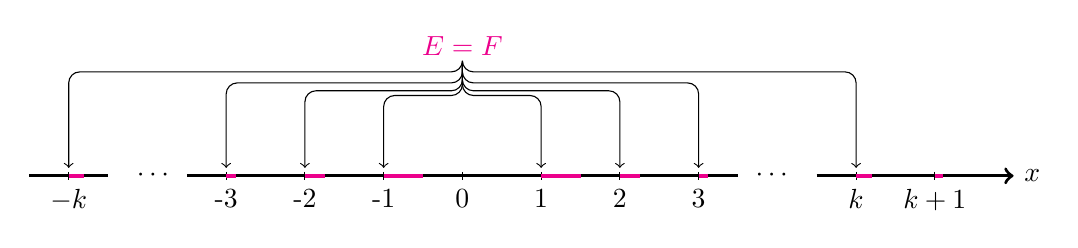
\begin{tikzpicture}
     \draw [very thick] (-3.5,0) -- (3.5,0);
     \draw (3.6,0) node[right] {$\cdots $} ;
     \draw [very thick,->] (4.5,0) -- (7.0,0) node [right] {$x$};
     \draw (-3.6,0) node[left] {$\cdots $};
     \draw [very thick] (-5.5,0) -- (-4.5,0);
     \foreach \x in {-3,...,3} \draw (\x,0.05) -- (\x,-0.05) node[below] {\x};
     \draw (5,0.05) -- (5,-0.05) node[below] {$k$};
     \draw (-5,0.05) -- (-5, -0.05) node[below] {$-k$};
     \draw (6,0.05) -- (6, -0.05) node[below] {$k+1$};
     \draw [ultra thick,color = magenta] (1,0) -- (1.5,0);
     \draw [ultra thick,color =magenta] (-1,0) -- (-0.5,0);
     \draw [ultra thick,color =magenta] (2,0) -- (2+1/4,0);
     \draw [ultra thick,color = magenta] (-2,0) -- (-2+1/4,0);
     \draw [ultra thick,color =magenta] (3,0) -- (3+1/8,0);
     \draw [ultra thick,color =magenta] (-3,0) -- (-3+1/8,0);
     \draw [ultra thick,color =magenta] (5,0)--(5.2,0);
     \draw [ultra thick,color =magenta] (-5,0) -- (-4.8,0);
     \draw [ultra thick,color =magenta] (6,0) -- (6.1,0);
     \foreach \x in {-3, -2,-1,1,2,3} \draw[->,rounded corners] (0,1.4) --(0,1+\x*\x /50) -- (\x,1+\x*\x /50) -- (\x, 0.1);
     \draw (0,1.4) node[above] {$\color{magenta}{E=F}$};
     \draw[->,rounded corners] (0,1.4) -- (0,1+4*4 /50) -- (5,1+4*4/50) -- (5,0.1);
     \draw[->,rounded corners] (0,1.4) -- (0,1+4*4/50)--(-5, 1+4*4/50) -- (-5,0.1);
   \end{tikzpicture}
 \end{figure}
\end{frame}
\begin{frame}{$\alpha$密度集}
  下一步是去除测度有限的限制,为了达到这一目的,我们在能观测不等式这个方向中第一次引入了$\alpha$ 密度集的概念:
  \begin{block}{定义: $\alpha$密度集}
    给定一个大于$0$的常数$\alpha$,一个可测集称为{\color{magenta}$\alpha$密度集},如果其满足如下的$\alpha$指数衰减条件
    \[
      \varlimsup_{x\to \infty}|A\cap [x,x+1]|\lesssim |x|^{-\alpha}.
    \] 
  \end{block}
  有了这一定义,我们便可以描述第二个主要结果.
\end{frame}
\begin{frame}{主要结果II}
  \begin{block}{$E$和 $F$均为同时包含在$(c,\infty)$或者$(-\infty,c)$上的$\alpha>5 /6$密度集,其中$c$为任意常数}
    \[
      \int_{\R}|u(t,x)|^2\,\mathrm{d}x\le C \left( \int_{\R\backslash \color{magenta}E}|u(t_1,x)|^2\,\mathrm{d}x+\int_{\R \backslash \color{magenta} F}|u(t_2,x)|^2\,\mathrm{d}x \right). 
    \] 
  \end{block}
  举例: ${\color{magenta}E=F=\bigcup_{k\in \N} \left[k,k+\frac{1}{2k^{5.1 /6}}\right]} $, 该集合测度是{\color{magenta}{无限}}的,分布如下图所示:
 \begin{figure}
   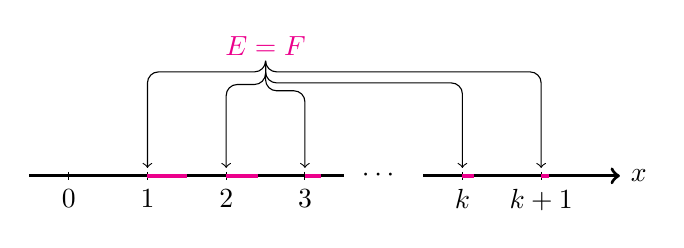
\begin{tikzpicture}
     \draw [very thick] (-0.5,0) -- (3.5,0);
     \draw (3.6,0) node[right] {$\cdots $};
     \draw [very thick,->] (4.5,0) --(7,0) node [right] {$x$};
     \foreach \x in {0,1,2,3} \draw (\x,0.05) -- (\x,-0.05) node[below] {\x};
     \draw (5,0.05)--(5,-0.05) node[below]{$k$};
     \draw (6,0.05)--(6,-0.05) node[below]{$k+1$};
     \draw [ultra thick,color=magenta] (1,0) -- (1.5,0);
     \draw [ultra thick, color=magenta] (2,0) -- (2.4,0);
     \draw [ultra thick,color=magenta] (3,0) -- (3.2,0);
     \draw [ultra thick,color=magenta] (5,0) -- (5.15,0);
     \draw [ultra thick,color=magenta] (6,0) -- (6.1,0);
     \draw [->, rounded corners] (2.5,1.4) -- (2.5,1+16 /50) -- (1,1+16/50) -- (1,0.1);
     \draw [->,rounded corners] (2.5,1.4) -- (2.5,1+8 /50) -- (2,1+8/50) -- (2,0.1);
     \draw [->, rounded corners] (2.5, 1.4) -- (2.5,1+4/50)--(3,1+4/50)--(3,0.1);
     \draw [->,rounded corners] (2.5,1.4) -- (2.5,1+9/50)--(5,1+9/50)--(5,0.1);
     \draw [->,rounded corners] (2.5,1.4)--(2.5,1+16/50)--(6,1+16/50)--(6,0.1);
     \draw (2.5,1.4) node[above] {$\color{magenta}{E=F}$};
   \end{tikzpicture}
 \end{figure}

\end{frame}


\begin{frame}{主要结果II}
实际上, ${\color{magenta}E}$和 ${\color{magenta}{F}}$所满足的密度条件可以放得更宽,可以表示为下图的有色区域:
  \begin{figure}
    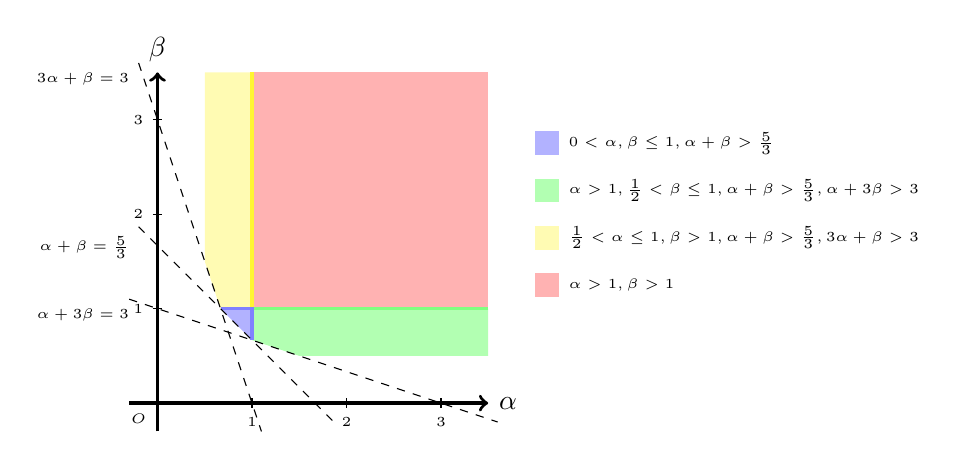
\begin{tikzpicture}[scale=1.2]
       % axes
       \draw[very thick,->] (-0.3,0) -- (3.5,0) node[right] {$\alpha$};
       \draw[very thick,->] (0,-0.3) -- (0,3.5) node[above] {$\beta$};
       % regions and boundaries
       \foreach \x in {1,...,3} \draw (\x, 0.05) -- (\x, -0.05) node[below] {\tiny \x};
       \foreach \y in {1,...,3} \draw (-0.05, \y) node[left] {\tiny \y} -- (0.05, \y);
       \fill[red!30] (1,1) -- (1,3.5) -- (3.5,3.5) -- (3.5,1) --cycle;
       \fill[yellow!30] (1/2,3/2) -- (2/3,1) -- (1,1) -- (1,3.5) --(1/2,3.5)--cycle;
       \fill[green!30] (3/2,1/2) -- (1,2/3) -- (1,1) -- (3.5,1) --(3.5,1/2)--cycle;
       \fill[blue!30] (2/3,1) -- (1, 2/3) -- (1,1) --cycle;
       \draw (-0.2,-0.01) node[below] {\tiny $O$};
       \draw[yellow!80, very thick] (1,1) -- (1,3.5);
       \draw[green!50, very thick] (1,1) -- (3.5,1);
       \draw[blue!50, very thick] (2/3,1)--(1,1)--(1,2/3);
       % labels
       \fill[blue!30] (4,3.25-0.625)--(4.25,3.25-0.625)--(4.25,3.5-0.625)--(4,3.5-0.625);
       \draw (4.25,3.375-0.625) node[right] {\tiny$0<\alpha,\beta\le 1,\alpha+\beta>\frac{5}{3}$};
       \fill[yellow!30] (4,2.25-0.625) -- (4.25,2.25-0.625) -- (4.25, 2.5-0.625) -- (4,2.5-0.625);
       \draw (4.25, 2.375-0.625) node[right] {\tiny$\frac{1}{2}<\alpha\le 1,\beta>1,\alpha+\beta>\frac{5}{3},3\alpha+\beta>3$};
       \fill[green!30] (4,2.75-0.625) -- (4.25, 2.75-0.625) -- (4.25,3-0.625)--(4,3-0.625);
       \draw (4.25,2.875-0.625) node[right] {\tiny$\alpha>1,\frac{1}{2}<\beta\le 1,\alpha+\beta>\frac{5}{3},\alpha+3\beta>3$};
       \fill[red!30] (4,1.75-0.625) -- (4.25, 1.75-0.625) -- (4.25,2-0.625) -- (4,2-0.625);
       \draw (4.25,1.875-0.625) node[right] {\tiny $\alpha>1,\beta>1$};
       % lines and equations
       \draw[dashed] (-1/5,18/5)node[below left]{\tiny $3\alpha+\beta=3$} --(1.1,-0.3);
       \draw[dashed] (-0.3,1.1)  --(18/5,-1/5);
       \draw (-1/5,1.1) node[below left]{\tiny $\alpha+3\beta=3$};
       \draw[dashed] (-1/5,28/15) node[below left]{\tiny $\alpha+\beta=\frac{5}{3}$}-- (28/15,-1/5);
    \end{tikzpicture}
    \end{figure}
\end{frame}
\begin{frame}{总结与展望}
  我们的主要工作是得到了线性KdV方程两个新的能观测不等式,具体地说,就是得到了非观测区域${\color{magenta}E}$和 ${\color{magenta}F}$取
  \begin{enumerate}
    \item[(1)] 具有有限测度的可测集(突破了{\color{magenta}有界}的限制)
    \item[(2)] 具有某种密度条件且处在同一半轴的可测集(突破了{\color{magenta}测度有限}的限制)
  \end{enumerate}
  两种情况下的{\color{red}两点时刻能观测不等式}并得以发表\footnote{Yunlei Wang, Ming Wang, Observability inequality at two time points for the KdV equation from measurable sets. J. Math. Anal. Appl. 505 (2022), no. 2, Paper No.125643, 15 pp, available online 2 September 2021.}.
  
  关于这个方向有许多有待解决的问题,例如计算出更加精确的控制常数$C$,或者去除处在同一半轴的限制等等,这些是接下来需要考虑的问题!
\end{frame}
\begin{frame}
  \begin{center}
    \Huge {\itshape The End!}
\end{center}
\end{frame}
